\documentclass{article}
\usepackage[utf8]{inputenc}
\usepackage[spanish]{babel}
\usepackage{float}
\usepackage[margin=2.5cm]{geometry}
\usepackage{graphicx}

\title{\textbf{Una imagen dice más que mil palabras... ¿y una figura?}}
\author{Verónica Jackeline Quiros Díaz}
\date{July 2020}
\begin{document}
\maketitle
\centering \listoffigures
%--------------------Original--------------------
\begin{center}
    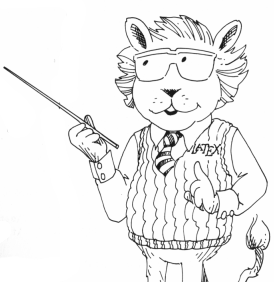
\includegraphics{images/latexlion2.png}
\end{center}
\newpage
%--------------------a--------------------
\begin{figure}[H]
    \centering
    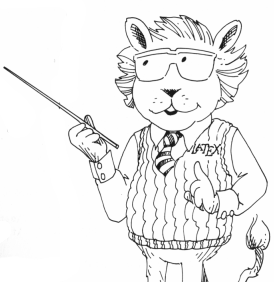
\includegraphics[width=2.5cm]{images/latexlion2.png}
    \caption{Imagen con width}
    \label{fig:my_label}
\end{figure}
%-------------------b----------------------
\begin{figure}[H]
    \centering
    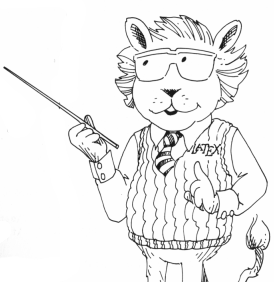
\includegraphics[height=7cm]{images/latexlion2.png}
    \caption{Imagen con height}
    \label{fig:my_label2}
\end{figure}
%-------------------c----------------------
\begin{figure}[H]
    \centering
    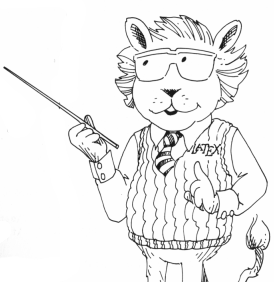
\includegraphics[width=0.5\textwidth]{images/latexlion2.png}
    \caption{Imagen con \textbackslash{}textwidth}
    \label{fig:my_label3}
\end{figure}
%-------------------d----------------------
\begin{figure}[H]
    \centering
    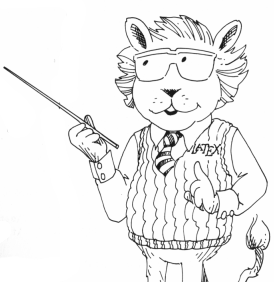
\includegraphics[width=2.5cm,height=4cm,keepaspectratio]{images/latexlion2.png}
    \caption{Imagen con keepaspectratio}
    \label{fig:my_label4}
\end{figure}
%-------------------e----------------------
\begin{figure}[H]
    \centering
    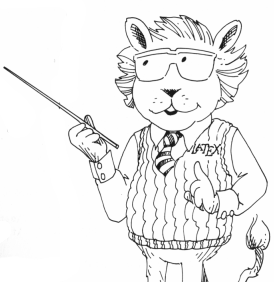
\includegraphics[scale=0.75]{images/latexlion2.png}
    \caption{Imagen con scale}
    \label{fig:my_label5}
\end{figure}
%-------------------f----------------------
\begin{figure}[H]
    \centering
    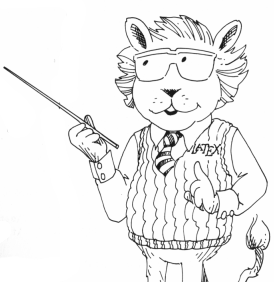
\includegraphics[draft]{images/latexlion2.png}
    \caption{Imagen con draft}
    \label{fig:my_label6}
\end{figure}
%-------------------g----------------------
\begin{figure}[H]
    \centering
    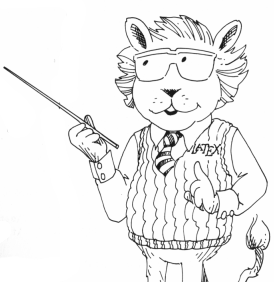
\includegraphics[angle=90]{images/latexlion2.png}
    \caption{Imagen con angle}
    \label{fig:my_label7}
\end{figure}
%-----------------------------------------
\newpage
\section{Explicación de Efectos}
\begin{itemize}
    \item width: Permite colocar el ancho de la imagen. Manejando diversas metricas, tales como: cm, mm, pm,etc. \textbf{Figura\ref{fig:my_label}} 
    \item height: En este caso, permite entablar el alto de la imagen, detallando la metrica que se quiera: cm, mm, pm, etc. \textbf{Figura \ref{fig:my_label2}} 
    \item \textbackslash{}textwidth: Permite modificar la escala, de acuerdo al tamaño de los margenes que se establezcan. \textbf{Figura \ref{fig:my_label3}} 
    \item keepaspectratio: Hace efecto cuando se establece \textit{width} y \textit{height}. Selecciona la medida menor y la aplica para ambas. \textbf{Figura \ref{fig:my_label4}} 
    \item scale: incrementa o decrementa la iamgen de acuerdo al tamaño que se defina en decimal $(50\%=0.5)$. \textbf{Figura \ref{fig:my_label5}} 
    \item draft: Muestra el recuadro que ocupa y direccion de la imagen. \textbf{Figura \ref{fig:my_label6}} 
    \item angle: La rotación que se le quiera dar: 45,90,etc. \textbf{Figura \ref{fig:my_label7}} 
\end{itemize}




\end{document}
